\chapter{Bảng Tuần Hoàn Các Nguyên Tố Hóa học}
\section{Các Xu Hướng Biến Đổi Trong Bảng Tuần Hoàn}
\begin{mtbh}
	\begin{itemize}
		\item Giải thích được xu hướng biến đổi bán kính nguyên tử trong một chu kì, trong một nhóm (các nguyên tố nhóm A).
		\item Nhận xét và giải thích được xu hướng biến đổi độ âm điện và tính kim loại, phi kim của nguyên tử các nguyên tố trong một chu kì, trong một nhóm (nhóm A).
		\item Nhận xét được xu hướng biến đổi thành phần và tính acid, tính base của các oxide và các hydroxide theo chu ki. Viết được phương trình hoá học minh hoạ.
	\end{itemize}
\end{mtbh}
\subsection{Xu Hướng biến đổi bán kính}
\begin{hoplythuyet}
	\noibat[\maunhan]{Trong một chu kì}
		Quy luật chung đối với các nguyên tố nhóm A: Trong một chu kì, theo chiều tăng dần điện tich hạt nhân, bán kính các nguyên tử có xu hướng giảm dần.
	\GSND[\bfseries\sffamily][\faKey]{Giải thích:}Trong một chu kì đi từ trái sang phải, nguyên tử các nguyên tố có cùng số lớp e nhưng khi điện tích tăng dần các electron chịu lực hút của hạt nhân càng lớn do đo bán kính của các nguyên tử co lại.
	\noibat[\maunhan]{Trong một nhóm A}
	Quy luật chung đối với các nguyên tố nhóm A: Trong một nhóm, theo chiều tăng diện tích hạt nhân, bán kính của nguyên tử có xu hướng tăng dần.
	\GSND[\bfseries\sffamily][\faKey]{Giải thích:}Trong một nhóm A đi từ trên xuống,mặc dù nguyên tử các nguyên tố có điện tích hạt nhân tăng dần tuy nhiên sự tăng số lớp e chiếm ưu thế nên tổng thể bán kính nguyên tử tăng dần.
\end{hoplythuyet}
\subsection{BÀI TẬP VỀ XU HƯỚNG BIẾN ĐỔI BÁN KÍNH}
\begin{dangntd}{Xu hướng biến đổi bán kính}
	\nhanmanh{Bài toán 1: So sánh bán kính nguyên tử}
	\GSND[\bfseries][\faBook][\maunhan]{Quy luât:}
%	\taodongke[\maunhan][1.12]{30}
	\begin{enumerate}
		\item Trong một \indam[\maudam]{chu kì} đi từ trái sang phải theo chiều tăng của điện tích hạt nhân bán kính nguyên tử \indam[\maudam]{giảm} dần
		\item Trong một \indam[\maudam]{nhóm A}, đi từ trên xuống dưới theo chiều tăng của điện tích hạt nhân bán kính nguyên tử \indam[\maudam]{tăng} dần
		\item Theo tổng thể \indam[\maudam]{tăng dần}  theo \indam[\maudam]{đường chéo bậc thang} kẻ từ \indam[\maudam]{góc trên bên phải} đến \indam[\maudam]{góc dưới bên trái} của bảng tuần hoàn
	\end{enumerate}
	\begin{center}
		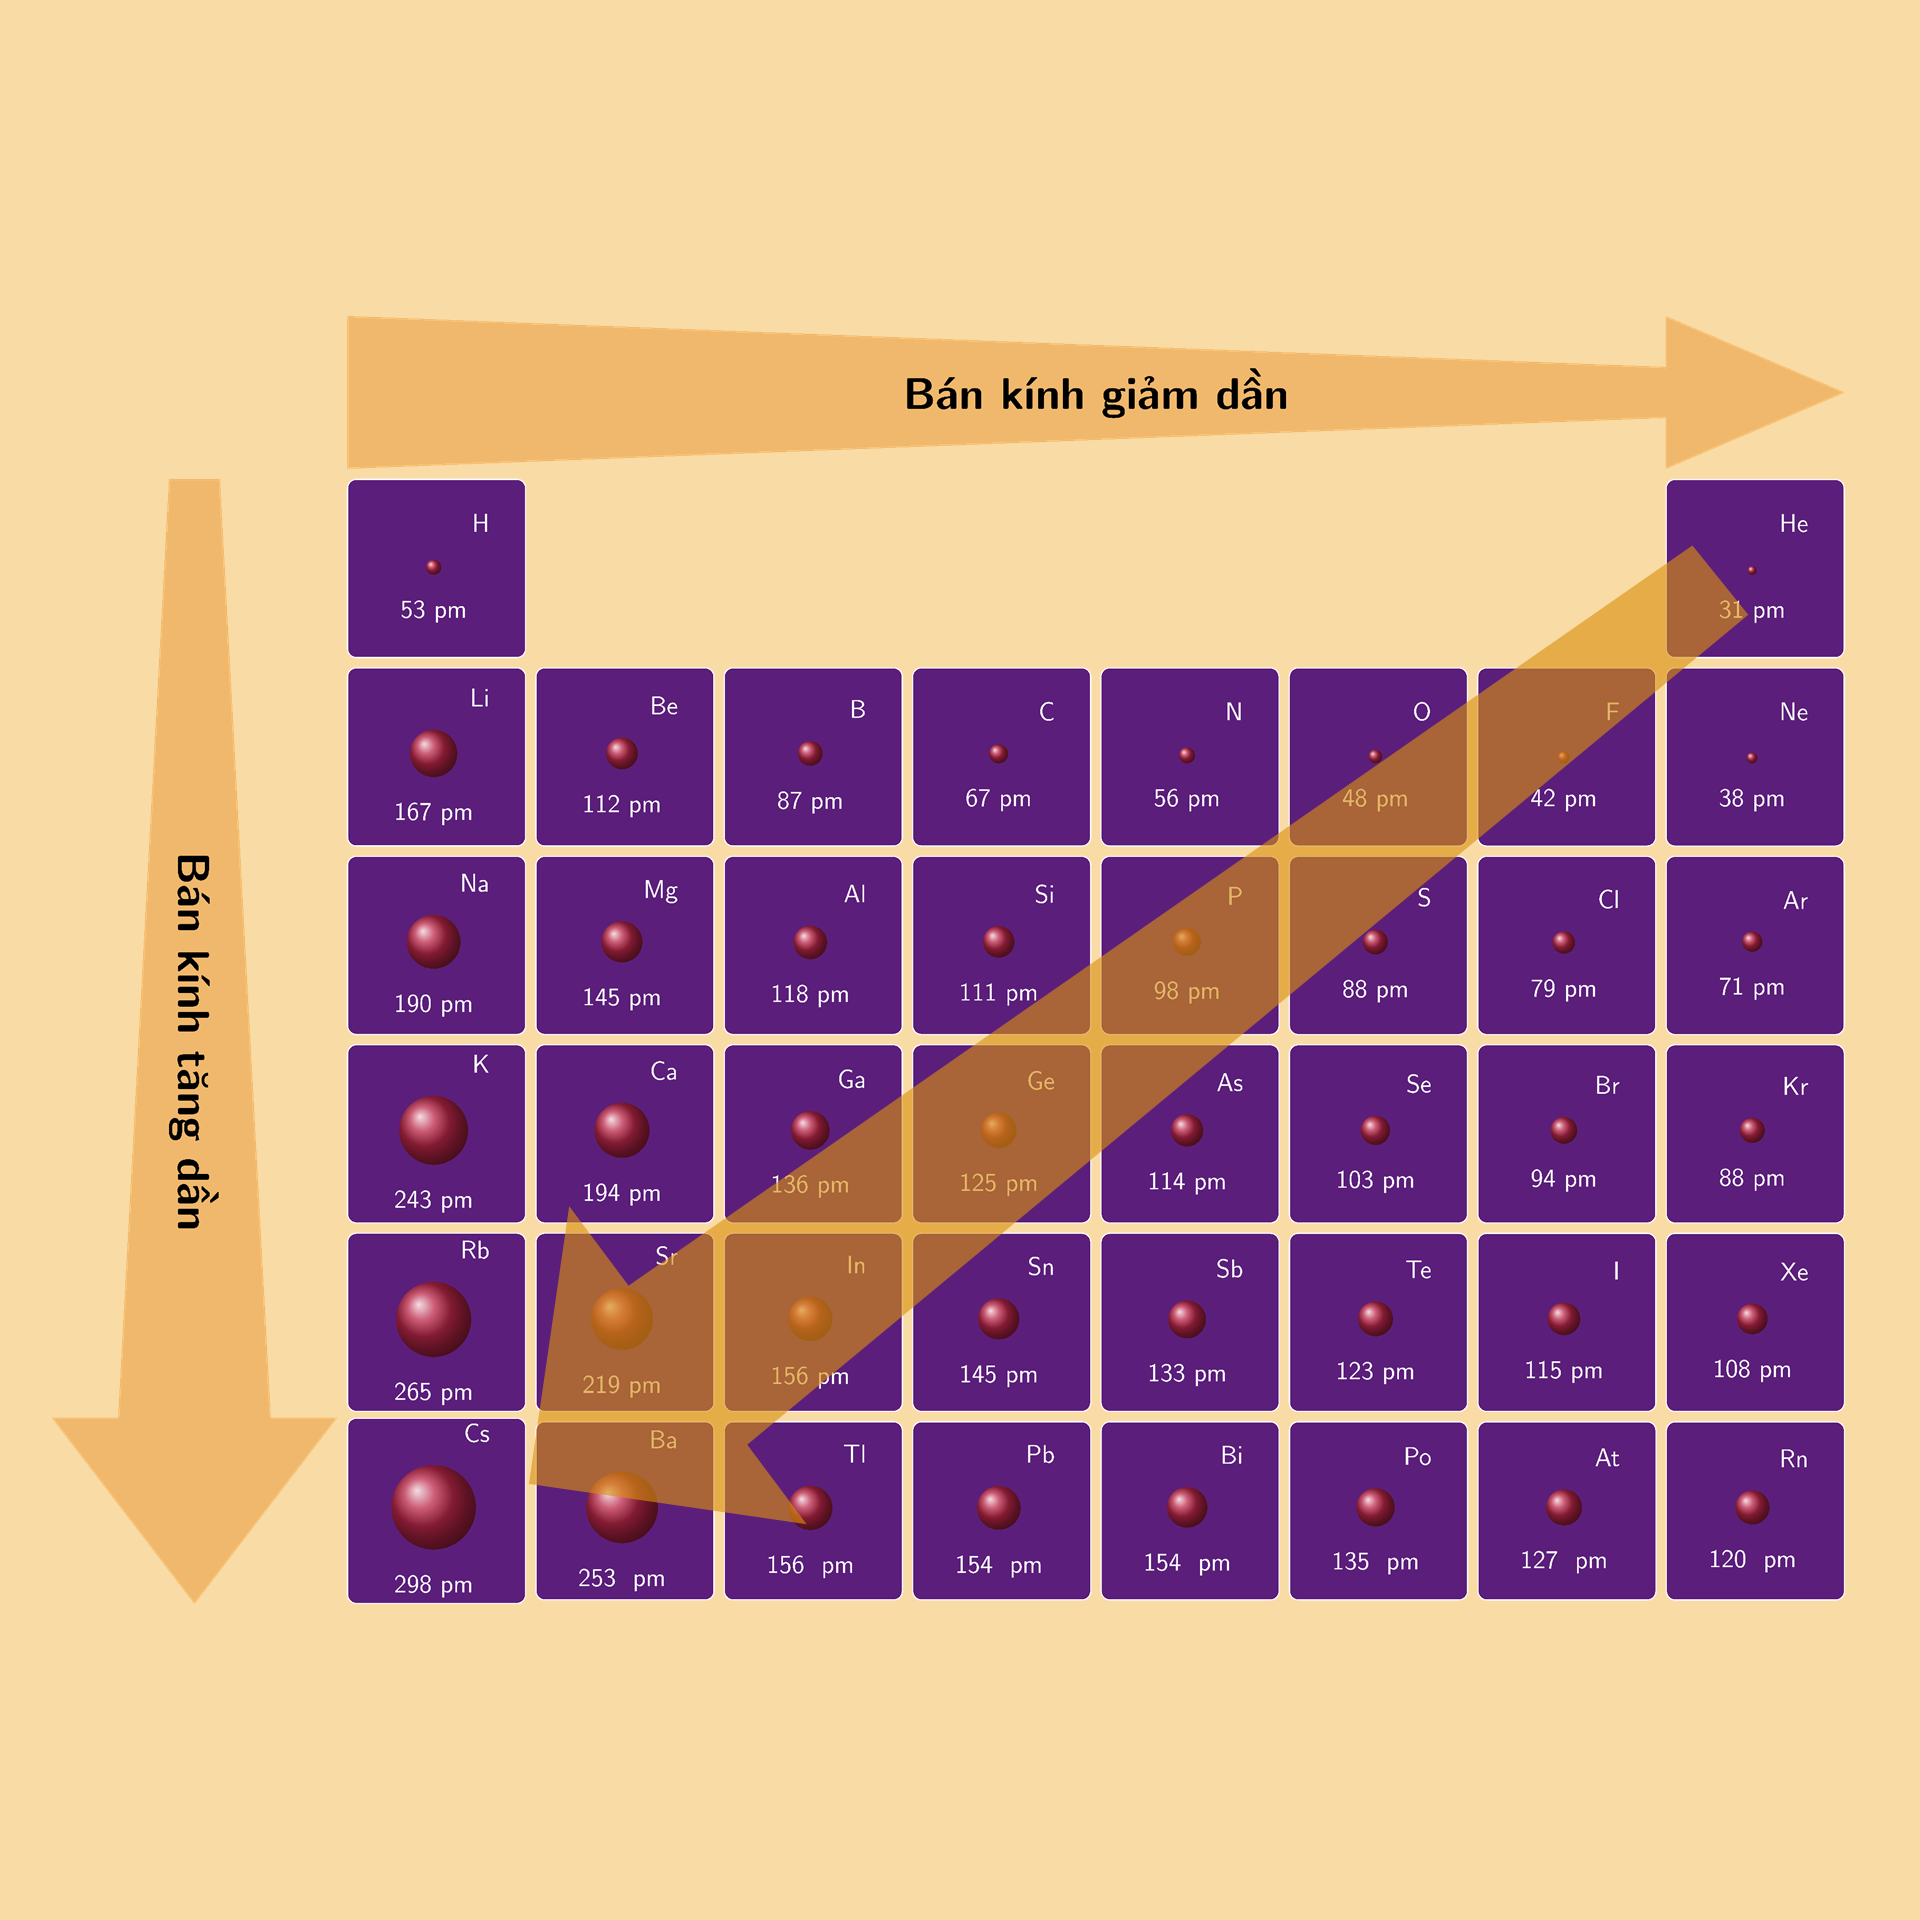
\includegraphics[width 	=8cm]{Images/anhminhoa/xuhuongbk.png}
	\end{center}
	\nhanmanh{Bài toán 2: So sánh bán kính ion}
	\GSND[\bfseries][\faBook][\maunhan]{Quy luât 1:}
%	\taodongke[\maunhan][1.12]{16}
	So với nguyên tử trung hòa
	\begin{enumerate}
		\item Khi một nguyên tử nhường e (cation) thì bán kính sẽ giảm đi
		\item Khi một nguyên tử nhận e (anion) thì bán kính nguyên tử sẽ tăng lên
	\end{enumerate}
	Do vây, đối với cùng nguyên tố thì:
	\begin{center}
		\boxct{Bán kính$_{cation}$ < bán kính $_{\text{nguyên tử}}$ < bán kính $_{anion}$}
	\end{center}
	\GSND[\bfseries][\faBook][\maunhan]{Quy luât 2:}
%	\taodongke[\maunhan][1.12]{18}
	Các ion có cùng số electron
	\begin{enumerate}
		\item Cation có điện tích càng lớn thì bán kính càng nhỏ
		\item Anion có điện tích càng lớn thì bán kính càng lớn
	\end{enumerate}
% \taodongke[\maunhan][1.12]{16}
\end{dangntd}
\newpage
\GSND[\bfseries][\faBookReader][\maudam]{Ví dụ mẫu:}
%%%==============VD_01===================%%%
\begin{vd}
	Hãy sắp xếp các nguyên tố $_{20}Ca$, $_{4}Be$, $_{12}Mg$ theo chiều tăng dần bán kính nguyên tử?
	\loigiai{
	Dựa vào  số hiệu nguyên tử các em viết cấu hình electron của các nguyên tử \Muiten{->} vị trí \Muiten{->} phác thảo lên bảng tuần hoàn  đưa ra quy luật biến đổi tính chất\\
	Ta có:\\
	$_{20}Ca: 1s^{2}2s^{2}2p^{6}3s^{2}3p^{6}4s^{2}$ \Muiten{->} Ca thuộc chu kì 4, nhóm IIA\\
	$_{4}Be: 1s^{2}2s^{2}$ \Muiten{->} Be thuộc chu kì 2, nhóm IIA\\
	$_{12}Mg: 1s^{2}2s^{2}2p^{6}3s^{2}$ \Muiten{->} Mg thuộc chu kì 3, nhóm IIA\\
	Ba nguyên tố Ca, Be, Mg thuộc cùng một nhóm nên chiều bán kính tăng dần là: Be < Mg < Ca
	}
\end{vd}
%%%==============VD_02===================%%%
\begin{vd}
	Hãy sắp xếp các nguyên tố $_{11}Na$, $_{17}Cl$, $_{15}P$, $_{13}Al$ theo chiều tăng dần bán kính nguyên tử?
	\sodongkevd[10]
\end{vd}
%%%==============VD_03===================%%%
\begin{vd}
	Hãy sắp xếp các nguyên tố $_{8}O$, $_{15}P$, $_{13}Al$, $_{20}Ca$, $_{19}K$ theo chiều tăng dần bán kính nguyên tử?
	\sodongkevd[10]
\end{vd}
%%%==============VD_04===================%%%
\begin{vd}
	Cho điện tích hạt nhân $O(Z=8), \mathrm{Na}(Z=11), \mathrm{Mg}(Z=12), \mathrm{Al}(Z=13)$ và các hạt vi mô: $O^{2-}, \mathrm{Al}^{3+}, \mathrm{Al}, \mathrm{Na}, \mathrm{Mg}^{2+}, \mathrm{Mg}$. Dãy nào sau đây được xếp đúng thứ tự bán kính hạt?
	\sodongkevd[15]
\end{vd}
%%%==============VD_05===================%%%
\begin{vd}
	Cho điện tích hạt nhân $O(Z=8), \mathrm{F}(Z=9), \mathrm{Mg}(Z=12), \mathrm{Al}(Z=13),\mathrm{S}(Z=16),\mathrm{Cl}(Z=17),\mathrm{K}(Z=19),\mathrm{Ca}(Z=20)$.Hãy sắp xếp dãy các ion sau: $\mathrm{S}^{2-},\mathrm{Cl}^{-},\mathrm{K}^{+},\mathrm{Ca}^{2+},\mathrm{Al}^{3+},\mathrm{Mg}^{2+},\mathrm{O}^{2-},\mathrm{F}^{-} $ theo chiều tăng dần của bán kính?
	\sodongkevd[15]
\end{vd}







